\documentclass[11pt]{article}
\usepackage[T1]{fontenc}
\usepackage{lmodern}
\usepackage{amsmath,amssymb,amsthm,mathtools}
\usepackage[letterpaper,margin=1in]{geometry}
\usepackage{microtype}
\usepackage{enumitem}
\usepackage{booktabs}
\usepackage{graphicx}
\usepackage{tikz}
\usetikzlibrary{arrows.meta,calc,positioning}
\usepackage{xcolor}
\definecolor{linkblue}{HTML}{23527C}
\definecolor{parentblue}{HTML}{28698D}
\definecolor{childorange}{HTML}{B76223}
\usepackage[colorlinks=true,linkcolor=linkblue,citecolor=linkblue,urlcolor=linkblue]{hyperref}
\usepackage[capitalise,noabbrev]{cleveref}
\hypersetup{pdftitle={Thompson's group F is nonamenable}}

\newcommand{\R}{\mathbb R}
\newcommand{\N}{\mathbb N}
\newcommand{\Z}{\mathbb Z}
\newcommand{\norm}[1]{\lVert #1\rVert}
\newcommand{\ip}[2]{\langle #1,#2\rangle}
\newcommand{\id}{\mathrm{id}}
\DeclareMathOperator{\Lip}{Lip}
\DeclareMathOperator{\dist}{dist}
\DeclareMathOperator{\colr}{col}
\DeclareMathOperator{\sinc}{sinc}
\DeclareMathOperator{\cvec}{cs}
\newcommand{\unverified}[1]{\par\smallskip\noindent\fbox{\parbox{0.95\linewidth}{\textbf{Unverified step.} #1}}\par\smallskip}
\newtheorem{theorem}{Theorem}[section]
\newtheorem{lemma}[theorem]{Lemma}
\newtheorem{proposition}[theorem]{Proposition}
\newtheorem{corollary}[theorem]{Corollary}
\theoremstyle{definition}
\newtheorem{definition}[theorem]{Definition}
\newtheorem{remark}[theorem]{Remark}
\numberwithin{equation}{section}
\setlist[itemize]{topsep=4pt,itemsep=2pt,parsep=0pt}
\setlist[enumerate]{topsep=4pt,itemsep=2pt,parsep=0pt}
\setlength{\emergencystretch}{2em}

\title{Thompson's group \(F\) is nonamenable}
\author{Rewritten for readability from the OpenAI manuscript of the same title}
\date{September 23, 2026}

\begin{document}
\maketitle
\begin{abstract}
We prove that Thompson's group \(F\) is nonamenable. This confirms
Geoghegan's conjecture and resolves the amenability problem for \(F\).
The proof is one finite averaging argument: a F\o lner set for a certain
fixed finite subset of \(F\) would produce an approximate fixed point of a
Lipschitz self-map of the Hilbert unit ball that has none.
\end{abstract}

\section{The result and how it is proved}\label{sec:introduction}

\subsection{Statement}

\emph{Thompson's group} \(F\) is the set of homeomorphisms
\(g:[0,1]\to[0,1]\) that are increasing and piecewise linear with finitely
many pieces, whose breakpoints are dyadic rationals (numbers \(k2^{-r}\)
with \(k,r\) integers), and whose slopes lie in
\(2^{\Z}=\{2^{\lambda}:\lambda\in\Z\}\). The product is composition,
\(hg=h\circ g\), and \(F\) is regarded as a discrete group.

A discrete group \(G\) is \emph{amenable} if there is a linear functional
\(\mu:\ell^\infty(G;\R)\to\R\) with \(\mu(1)=1\), \(\mu(\psi)\ge0\) whenever
\(\psi\ge0\), and \(\mu(g\mapsto\psi(hg))=\mu(\psi)\) for every \(h\in G\).
This invariant-mean viewpoint belongs to the classical theory of von Neumann
and Day \cite{vonNeumann1929,Day1957}. We use only the forward implication
of the F\o lner criterion \cite{Folner1955}:

\begin{quote}
\emph{If \(G\) is amenable, then for every finite \(S\subset G\) and every
\(\varepsilon>0\) there is a nonempty finite \(A\subset G\) such that}
\begin{equation}\label{eq:folner}
  \frac{|hA\mathbin{\triangle}A|}{|A|}<\varepsilon
  \qquad\text{for every } h\in S .
\end{equation}
\end{quote}
Here \(hA=\{ha:a\in A\}\) and \(\triangle\) is symmetric difference. The
source takes \eqref{eq:folner} from the left-translation formulation in
\cite[Theorem~1.2]{Moore2013}, which, as the source reports it, bounds the
\emph{sum} over \(h\in S\) of these ratios. Each ratio is nonnegative, hence
at most the sum, and applying that formulation with tolerance
\(\varepsilon/2\) gives the strict bound \eqref{eq:folner} for each
\(h\) separately.

\begin{theorem}\label{thm:main}
Thompson's group \(F\) is not amenable.
\end{theorem}

What is actually proved is quantitative (\cref{avg:boundary}): there are a
finite set \(S\subset F\) and a constant \(c_0>0\) such that
\(\max_{h\in S}|hA\mathbin{\triangle}A|/|A|\ge c_0\) for \emph{every}
nonempty finite \(A\subset F\). This contradicts \eqref{eq:folner} with
\(\varepsilon=c_0\).

\subsection{The one analytic input}

\begin{lemma}[Benyamini--Sternfeld]\label{lem:displacement}
There are a real Hilbert space \(H\), a Lipschitz map \(f:B\to B\) on its
closed unit ball \(B\), and a constant \(\delta>0\) such that
\[
  \norm{f(x)-x}\ge\delta\qquad(x\in B).
\]
\end{lemma}

Benyamini and Sternfeld prove this for every infinite-dimensional normed
space \cite[Theorem, part~(3), p.~439]{BenyaminiSternfeld1983}.
\Cref{app:auxiliary} gives a self-contained construction on
\(L^2([0,1];\R^2)\) with \(\delta=1/2\). The lemma is used in
\cref{sec:coloring} to define the coloring and in Step~4 of the proof of
\cref{avg:boundary}. No such \(f\) exists when \(\dim H<\infty\), by
Brouwer's fixed-point theorem, so infinite dimension is essential.

\subsection{Proof at a glance}\label{sec:glance}

\paragraph{Objects.}
Fix \(f,L,\delta\) as in \cref{lem:displacement} (\(L\) a Lipschitz constant
of \(f\)) and an integer \(D>4L^2/\delta^2\). A \emph{basic interval} is a
dyadic interval \([k2^{-r},(k+1)2^{-r}]\subseteq[0,1]\). For a basic
interval \(I\), \(s_I:[0,1]\to I\) is the increasing affine bijection.
\begin{itemize}
\item \emph{Parents:} \(D\) basic intervals \(I_1<\dots<I_D\) inside
\((0,1)\) with positive gaps between consecutive ones.
\item \emph{Children:} the \(D^2\) intervals \(I_i\cdot I_j:=s_{I_i}(I_j)\),
that is, the same family \(I_1<\dots<I_D\) copied affinely into each parent
\(I_i\). (The source calls them descendants.)
\item \emph{Colors:} to each finite partition \(T\) of \([0,1]\) into basic
intervals we attach a vector \(\colr(T)\in B\) by recursion: if every parent
is a union of cells of \(T\), then \(\colr(T)\) is \(f\) applied to the
average of the colors of the \(D\) partitions that \(T\) induces on the
parents, each stretched back to \([0,1]\); otherwise \(\colr(T)=0\).
\item \emph{Functions on \(F\):} for \(g\in F\) and a fine uniform dyadic
partition \(T^{(n)}\), let \(X_I(g)\) be the color of the partition
\(gT^{(n)}\) restricted to \(I\) and stretched back to \([0,1]\), for \(I\) a
parent or a child. By construction
\[
 X_{I_i}(g)=f(z_i(g)),\qquad
 z_i(g)=\frac1D\sum_{j=1}^D X_{I_i\cdot I_j}(g),\qquad
 m(g)=\frac1D\sum_{i=1}^D X_{I_i}(g).
\]
\end{itemize}

\paragraph{Key idea.}
Let \(A\subset F\) be finite and think of \(g\) as uniformly random in \(A\).
\begin{enumerate}[label=(\roman*)]
\item \emph{Group theory.} \(F\) contains, for each pair \(I<J\) of disjoint
parents or children with a positive gap, an element \(h_{I,J}\) mapping \(I\)
affinely onto \(I_1\) and \(J\) affinely onto \(I_2\). Colors are carried
along exactly: \(X_I(g)=X_{I_1}(h_{I,J}g)\) and \(X_J(g)=X_{I_2}(h_{I,J}g)\).
If \(A\) is almost invariant under the finite set \(S\) of these elements,
with defect \(\eta\), then the average over \(A\) of \(\ip{X_I}{X_J}\) is
within \(\eta\) of one number \(\alpha\) for all such pairs. The number
\(\alpha\) depends on \(A\), but not on the pair.
\item \emph{Hilbert space.} Vectors whose pairwise correlations all equal
\(\alpha\) behave like one common vector plus uncorrelated noise, so any two
averages of \(D\) of them nearly agree. Precisely,
\(\mathbb E_A\norm{z_i-m}^2\le 4/D+4\eta\).
\item \emph{Contradiction.} Since \(m\) is the average of the \(f(z_i)\) and
\(f\) is \(L\)-Lipschitz, (ii) gives
\(\mathbb E_A\norm{m-f(m)}^2\le L^2(4/D+4\eta)\). But
\(\norm{m-f(m)}\ge\delta\) always. Hence \(\eta\) is bounded below by a
positive constant independent of \(A\).
\end{enumerate}

\paragraph{Steps and dependencies.}
\begin{center}
\begin{tabular}{@{}lll@{}}
\toprule
Statement & Content & Used in\\
\midrule
\cref{lem:displacement} & the map \(f\) (proved in \cref{app:auxiliary}) &
   definition of \(\colr\); Step 4\\
\cref{dyad:restrict} & restriction is compatible with nesting &
   definition of \(\colr\); Step 3\\
\cref{dyad:eventual} & \(gT^{(n)}\) is basic and fine for large \(n\) & Step 0\\
\cref{dyad:transport} & pair transport in \(F\) & definition of \(S\)\\
\cref{dyad:covariancelemma} & transports preserve restricted partitions & Step 1\\
\cref{avg:translation} & averages over \(A\) and \(hA\) differ by the boundary & Step 2\\
\cref{avg:boundary} & uniform boundary bound (Steps 0--7) & \cref{thm:main}\\
\bottomrule
\end{tabular}
\end{center}
Inside the proof of \cref{avg:boundary}: Steps 1--2 give the correlation
comparison (i); Step 3 gives \(X_{I_i}=f(z_i)\); Step 4 is the pointwise
inequality in (iii); Steps 5--6 are (ii); Step 7 combines them.

\paragraph{Order of choices.}
\(f,L,\delta,D\), the parents, the children and the finite set \(S\) are
fixed once. Then \(A\) is arbitrary. Only the partition level \(n\), and
hence the number \(\alpha\), depend on \(A\).

\subsection{Context and prior work}

Thompson introduced \(F\) in 1965; an early published construction appears
in McKenzie and Thompson \cite{McKenzieThompson1973}, with the identification
explained by Cannon, Floyd, and Parry
\cite[pp.~215--216]{CannonFloydParry1996}, who also record Geoghegan's 1979
conjecture that \(F\) is nonamenable \cite[p.~227]{CannonFloydParry1996}.
Two classical tests are silent: \(F\) contains no nonabelian free subgroup
\cite[Theorem~3.1]{BrinSquier1985}, yet it is not elementary amenable
\cite[Theorem~4.10]{CannonFloydParry1996}. Brown and Geoghegan construct a
classifying space for \(F\) with finitely many cells in each dimension
\cite{BrownGeoghegan1984}. Moore proves tower lower bounds on the sizes of
F\o lner sets \cite[Theorem~1.1]{MooreFolner2013} and characterizes
amenability of \(F\) by a scalar convex Ramsey property for finite rooted
ordered binary trees \cite[Theorem~3.1]{Moore2013}. Guba improves densities
of finite Cayley subgraphs \cite{Guba2025Density} and derives restrictions on
right-invariant means \cite{Guba2026}. Haagerup and Olesen prove that
simplicity of the reduced \(C^*\)-algebra of Thompson's group \(T\) would
imply nonamenability of \(F\) \cite[Theorem~5.5]{HaagerupOlesen2017}. There
have been claims of a complete resolution in both directions: Akhmedov's 2021
version claims nonamenability through a height-function criterion
\cite{Akhmedov2021}; Shavgulidze claimed amenability \cite{Shavgulidze2009},
and Moore identified errors in that approach \cite{Moore2011Critique}; Moore
separately withdrew an amenability claim after Akhmedov identified an error
in Lemma~4.13 of that manuscript \cite{Moore2012Withdrawn} (a different work
from the Ramsey characterization above). None of these results is used below.
The proof uses only the standard dyadic-partition model of \(F\)
\cite[Section~2, Lemma~2.2]{CannonFloydParry1996}, and the facts needed from
it are proved in \cref{sec:dyadic}.

\subsection{Notation changed from the source}

To give every symbol one meaning, the following were renamed. The color map
\(p\) is now \(\colr\), because \(p\) is a percolation parameter in
\cref{sec:consequences}. The invariant mean \(M\) is now \(\mu\). The finite
set \(K\subset F\) in \cref{dyad:eventual} is now \(E\). In
\cref{sec:consequences} the Hilbert space and operator of
\cref{cor:nonunitarizable} are \(\mathcal H\) and \(V\), the generating set
is \(\Sigma\) (the letter \(S\) is reserved for the transport set), the
Cayley graph is \(\mathrm{Cay}(F,\Sigma)\), and the connection kernel is
\(\mathcal C_p\). In \cref{app:auxiliary} the map \(G\) is now \(\Phi\), the
operator \(A\) is \(\Lambda\), the quarter-turn \(J\) is written
\(\xi\mapsto\xi^\perp\), the second curve parameter \(s\) is \(\tau\), the
constants \(K,M\) are \(K_\gamma,M_\gamma\), and \(\norm{e}\) is written out
instead of being abbreviated \(r\).

\section{Proof of the theorem}\label{sec:proof}

\subsection{Dyadic partitions, restriction, and transport}\label{sec:dyadic}

\paragraph{Definitions.}
\begin{itemize}
\item A \emph{basic interval} is
\([k2^{-r},(k+1)2^{-r}]\subseteq[0,1]\) with \(r\in\N\cup\{0\}\) and
\(0\le k<2^r\); \(r\) is its \emph{level} and \(2^{-r}\) its length.
\item A \emph{basic partition} is a finite set \(T\) of basic intervals
(its \emph{cells}) with union \([0,1]\) and pairwise disjoint interiors.
\(|T|\) is the number of cells; the \emph{mesh} is the greatest cell length.
\item \(T\) \emph{respects} an interval \(I\) if \(I\) is a union of cells of
\(T\).
\item For intervals, \(I<J\) means \(\max I<\min J\) (a positive gap is
required). Two intervals are \emph{separated} if \(I<J\) or \(J<I\). An
interval is \emph{internal} if both endpoints lie in \((0,1)\).
\item For a basic interval \(I\), \(s_I:[0,1]\to I\) is the increasing affine
bijection, and \(I\cdot J:=s_I(J)\) for \(J\subseteq[0,1]\).
\item If \(T\) respects \(I\), its \emph{normalized restriction} is
\(T_I=\{s_I^{-1}(C):C\in T,\ C\subseteq I\}\).
\item \(T^{(n)}\) is the partition of \([0,1]\) into the \(2^n\) basic
intervals of level \(n\). For \(g\in F\),
\(gT^{(n)}=\{g(C):C\in T^{(n)}\}\).
\end{itemize}

\paragraph{Nesting fact.}
\emph{If two basic intervals have intersecting interiors, one contains the
other.} Let their levels be \(r\le r'\). The endpoints of the level-\(r\)
interval \(I\) are multiples of \(2^{-r'}\), so neither lies in the interior
of the level-\(r'\) interval \(I'\). An open interval that meets the interior
of \(I\) and contains no endpoint of \(I\) lies inside \(I\); hence
\(I'\subseteq I\).

\begin{lemma}[Restriction]\label{dyad:restrict}
Let \(I\) be a basic interval and \(T\) a basic partition respecting \(I\).
\begin{enumerate}[label=(\alph*)]
\item If \(J\) is a basic interval, then \(I\cdot J\) is a basic interval
contained in \(I\), and \(s_{I\cdot J}=s_I\circ s_J\).
\item \(T_I\) is a basic partition, and \(|T_I|\) is the number of cells of
\(T\) contained in \(I\). If \(I\) is internal, then \(|T_I|<|T|\).
\item If \(T\) also respects \(I\cdot J\) for a basic interval \(J\), then
\(T_I\) respects \(J\) and
\begin{equation}\label{dyad:restriction}
  (T_I)_J=T_{I\cdot J}.
\end{equation}
\end{enumerate}
\end{lemma}
This is used to see that the coloring recursion is well founded (b) and to
derive the identity \(X_{I_i}=f(z_i)\) in Step~3 below (c).

\begin{proof}
Write \(I=[l2^{-r},(l+1)2^{-r}]\), so \(s_I(x)=2^{-r}(x+l)\) and
\(s_I^{-1}(x)=2^rx-l\).

(a) If \(J=[k2^{-r'},(k+1)2^{-r'}]\), then
\(s_I(J)=[(k+l2^{r'})2^{-(r+r')},(k+1+l2^{r'})2^{-(r+r')}]\), a basic
interval of level \(r+r'\), contained in \(s_I([0,1])=I\). The map
\(s_I\circ s_J\) is an increasing affine bijection of \([0,1]\) onto
\(s_I(J)=I\cdot J\); such a bijection is unique, so it equals
\(s_{I\cdot J}\).

(b) Let \(C=[k2^{-r'},(k+1)2^{-r'}]\) be a cell of \(T\) with
\(C\subseteq I\). Its length is at most that of \(I\), so \(r'\ge r\), and
\[
 s_I^{-1}(C)=\bigl[(k-l2^{r'-r})2^{-(r'-r)},\,(k+1-l2^{r'-r})2^{-(r'-r)}\bigr]
 \subseteq[0,1]
\]
is a basic interval of level \(r'-r\). Since \(T\) respects \(I\), the cells
of \(T\) inside \(I\) have union \(I\) and disjoint interiors; the
homeomorphism \(s_I^{-1}:I\to[0,1]\) carries them to a basic partition, with
one cell for each. If \(I\) is internal, the cell of \(T\) containing \(0\)
is not inside \(I\), so \(|T_I|<|T|\).

(c) \(I\cdot J\) is a union of cells of \(T\). These cells lie in
\(I\cdot J\subseteq I\), so their images under \(s_I^{-1}\) are cells of
\(T_I\), with union \(s_I^{-1}(I\cdot J)=J\). Thus \(T_I\) respects \(J\).
Using (a) in the form \(s_J^{-1}\circ s_I^{-1}=s_{I\cdot J}^{-1}\) and
\(s_I^{-1}(C)\subseteq J\iff C\subseteq I\cdot J\),
\[
 (T_I)_J=\{s_J^{-1}(s_I^{-1}(C)):C\in T,\ C\subseteq I,\ s_I^{-1}(C)\subseteq J\}
 =\{s_{I\cdot J}^{-1}(C):C\in T,\ C\subseteq I\cdot J\}=T_{I\cdot J}.
 \qedhere
\]
\end{proof}

\begin{lemma}[Fine images are basic]\label{dyad:eventual}
\begin{enumerate}[label=(\alph*)]
\item For each \(g\in F\) there is \(n_g\) such that \(gT^{(n)}\) is a basic
partition for all \(n\ge n_g\); the mesh of \(gT^{(n)}\) tends to \(0\) as
\(n\to\infty\).
\item Given a finite set \(E\subset F\) and a finite family \(\mathcal J\) of
basic intervals, there is \(n_0\) such that \(gT^{(n)}\) is basic and respects
every member of \(\mathcal J\) whenever \(g\in E\) and \(n\ge n_0\).
\end{enumerate}
\end{lemma}
Part (b) is used once, in Step~0 of the proof of \cref{avg:boundary}.

\begin{proof}
(a) Let \(0=x_0<x_1<\dots<x_M=1\) be dyadic points such that
\(g(x)=2^{\lambda_i}x+\nu_i\) on \([x_{i-1},x_i]\), with \(\lambda_i\in\Z\).
Each \(g(x_i)\) is dyadic, by induction from \(g(x_0)=0\) and
\(g(x_i)=g(x_{i-1})+2^{\lambda_i}(x_i-x_{i-1})\). Hence
\(\nu_i=g(x_{i-1})-2^{\lambda_i}x_{i-1}\) is dyadic. Choose an integer
\(N\ge0\) such that all \(x_i\) and all \(\nu_i\) are integer multiples of
\(2^{-N}\), and put \(n_g=N+\max_i|\lambda_i|\). Let \(n\ge n_g\).
\begin{itemize}
\item Since \(n\ge N\), every \(x_i\) is a multiple of \(2^{-n}\), so each
cell \(C=[k2^{-n},(k+1)2^{-n}]\) of \(T^{(n)}\) lies in one piece
\([x_{i-1},x_i]\).
\item For such a cell,
\(g(C)=[k'2^{-(n-\lambda_i)},(k'+1)2^{-(n-\lambda_i)}]\) with
\(k'=k+\nu_i2^{\,n-\lambda_i}\). Here \(n-\lambda_i\ge N\ge0\), and \(k'\) is
an integer because \(\nu_i\in2^{-N}\Z\) and \(n-\lambda_i\ge N\). Since
\(g(C)\subseteq[0,1]\), it is a basic interval.
\item \(g\) is an increasing homeomorphism of \([0,1]\), so the intervals
\(g(C)\) have union \([0,1]\) and disjoint interiors.
\end{itemize}
Thus \(gT^{(n)}\) is a basic partition, of mesh at most
\(2^{\max_i\lambda_i-n}\to0\).

(b) Let \(\ell_0\) be the smallest length of a member of \(\mathcal J\). By
(a), for each \(g\in E\) there is \(n'_g\ge n_g\) with mesh of \(gT^{(n)}\)
less than \(\ell_0\) for \(n\ge n'_g\); let \(n_0=\max_{g\in E}n'_g\). Fix
\(g\in E\), \(n\ge n_0\), \(I\in\mathcal J\), and put \(T=gT^{(n)}\). Let
\(x\) be an interior point of \(I\) and \(C\) a cell of \(T\) containing
\(x\). Since \(x\) lies in the closure of the interior of \(C\), the interiors
of \(C\) and \(I\) meet. By the nesting fact one contains the other, and \(C\)
is shorter than \(I\), so \(C\subseteq I\). Hence the cells of \(T\) contained
in \(I\) cover the interior of \(I\), and, their union being closed, they
cover \(I\). So \(T\) respects \(I\).
\end{proof}

\begin{lemma}[Pair transport]\label{dyad:transport}
If \(I<J\) and \(I'<J'\) are pairs of internal basic intervals, there is
\(h\in F\) with \(h(I)=I'\), \(h(J)=J'\), and \(h\) affine on \(I\) and on
\(J\).
\end{lemma}
This is the only place where the structure of \(F\) beyond
\cref{dyad:eventual} is used. It supplies the finite set \(S\) in
\cref{sec:boundary}.

\begin{proof}
\emph{Step 1 (gaps).} The complement of \(I\cup J\) in \([0,1]\) consists of
three gaps: left of \(I\), between \(I\) and \(J\), and right of \(J\). Their
closures \(\Gamma_0,\Gamma_1,\Gamma_2\) have positive length (internality and
\(I<J\)) and dyadic endpoints. Define
\(\Gamma'_0,\Gamma'_1,\Gamma'_2\) likewise for \(I'<J'\). Choose \(N\) so
large that all endpoints of all these intervals are multiples of \(2^{-N}\).
Then each \(\Gamma_i\) is a union of \(p_i\ge1\) basic intervals of level
\(N\), and each \(\Gamma'_i\) of \(p'_i\ge1\) such intervals.

\emph{Step 2 (equalize counts).} Replacing a basic interval by its two halves
gives two basic intervals and raises the count by one. For each
\(i\in\{0,1,2\}\), perform \(|p_i-p'_i|\) such bisections on whichever of
\(\Gamma_i,\Gamma'_i\) has fewer cells. Now \(\Gamma_i\) and \(\Gamma'_i\) are
each divided into the same number \(P_i\) of basic intervals.

\emph{Step 3 (define \(h\)).} Listing from left to right the \(P_0\) cells of
\(\Gamma_0\), then \(I\), then the \(P_1\) cells of \(\Gamma_1\), then \(J\),
then the \(P_2\) cells of \(\Gamma_2\) gives a basic partition
\(C_1,\dots,C_Q\) of \([0,1]\), with \(Q=P_0+P_1+P_2+2\). The same recipe for
the primed data gives \(C'_1,\dots,C'_Q\), with \(I'\) in the same position as
\(I\) and \(J'\) in the same position as \(J\). Let \(h\) map each \(C_k\)
onto \(C'_k\) by the increasing affine bijection.

\emph{Step 4 (\(h\in F\)).} The right endpoint of \(C_k\) is the left
endpoint of \(C_{k+1}\), and both definitions send it to the common endpoint
of \(C'_k\) and \(C'_{k+1}\); so \(h\) is a well-defined increasing
homeomorphism of \([0,1]\). It is piecewise linear with at most \(Q\) pieces,
its breakpoints are endpoints of basic intervals and hence dyadic, and its
slope on \(C_k\) is \(|C'_k|/|C_k|\), a ratio of two powers of \(2\) since
every \(C_k\) and \(C'_k\) is basic. So \(h\in F\), and by construction \(h\)
maps \(I\) affinely onto \(I'\) and \(J\) affinely onto \(J'\).
\end{proof}

\begin{lemma}[Exact covariance]\label{dyad:covariancelemma}
Let \(I,I'\) be basic intervals and \(h\in F\) with \(h(I)=I'\) and \(h\)
affine on \(I\). Let \(g\in F\) and \(n\) be such that \(gT^{(n)}\) and
\((hg)T^{(n)}\) are basic partitions respecting \(I\) and \(I'\),
respectively. Then, as sets of intervals,
\begin{equation}\label{dyad:covariance}
  \bigl((hg)T^{(n)}\bigr)_{I'}=(gT^{(n)})_I .
\end{equation}
\end{lemma}
This is used in Step~1 of the proof of \cref{avg:boundary}.

\begin{proof}
The map \(h\circ s_I\) is an increasing affine bijection of \([0,1]\) onto
\(I'\), hence equals \(s_{I'}\); equivalently
\(s_{I'}^{-1}\circ h=s_I^{-1}\) on \(I\). Because \(hg=h\circ g\), the cells
of \((hg)T^{(n)}\) are exactly the sets \(h(C)\) with \(C\) a cell of
\(gT^{(n)}\). Since \(h\) is a bijection with \(h(I)=I'\), we have
\(h(C)\subseteq I'\iff C\subseteq I\). Therefore
\[
 \bigl((hg)T^{(n)}\bigr)_{I'}
 =\{s_{I'}^{-1}(h(C)):C\in gT^{(n)},\ C\subseteq I\}
 =\{s_I^{-1}(C):C\in gT^{(n)},\ C\subseteq I\}
 =(gT^{(n)})_I.\qedhere
\]
\end{proof}

\subsection{The recursive coloring}\label{sec:coloring}

\paragraph{Parameters (fixed for the rest of \cref{sec:proof}).}
Fix a real Hilbert space \(H\), its closed unit ball \(B\), a map
\(f:B\to B\), and constants \(L>0\), \(\delta>0\) such that
\begin{equation}\label{color:map}
  \norm{f(x)-f(y)}\leq L\norm{x-y},\qquad
  \norm{f(x)-x}\geq\delta
  \quad(x,y\in B);
\end{equation}
these exist by \cref{lem:displacement}. Fix an integer \(D\geq2\) with
\begin{equation}\label{color:parameters}
  D>\frac{4L^2}{\delta^2}.
\end{equation}
Fix internal basic intervals \(I_1<\cdots<I_D\) (the \emph{parents}). They
exist: take \(r\) with \(2^r>2D\) and \(I_j=[(2j-1)2^{-r},2j2^{-r}]\). Then
\(0<2^{-r}\le\min I_j\), \(\max I_j\le2D2^{-r}<1\), and
\(\max I_j=2j2^{-r}<(2j+1)2^{-r}=\min I_{j+1}\).

\paragraph{The color of a partition.}
Define \(\colr(T)\in B\) for every basic partition \(T\) by
\begin{equation}\label{color:recursion}
  \colr(T)=
  \begin{cases}
  \displaystyle f\left(\frac1D\sum_{j=1}^D \colr(T_{I_j})\right),
       &\text{if $T$ respects every $I_j$},\\[6pt]
  0,   &\text{otherwise}.
  \end{cases}
\end{equation}
\emph{This is well defined, by strong induction on \(|T|\).} Suppose
\(\colr(T')\in B\) is defined for all basic partitions with \(|T'|<|T|\). If
\(T\) does not respect every \(I_j\), then \(\colr(T)=0\in B\). Otherwise each
\(T_{I_j}\) is a basic partition with \(|T_{I_j}|<|T|\) by
\cref{dyad:restrict}(b), since \(I_j\) is internal. So each
\(\colr(T_{I_j})\in B\) is defined, their average lies in the convex set
\(B\), which is the domain of \(f\), and \(\colr(T)\in B\).

\emph{Example} (for the displayed choice of \(I_j\); not used later). The
one-cell partition \(T^{(0)}\) respects no \(I_j\), so \(\colr(T^{(0)})=0\).
Each \(I_j\) is a cell of \(T^{(r)}\) and \((T^{(r)})_{I_j}=T^{(0)}\), so
\(\colr(T^{(r)})=f(0)\). Likewise \((T^{(2r)})_{I_j}=T^{(r)}\), so
\(\colr(T^{(2r)})=f(f(0))\).

\paragraph{Parents and children.}
Let
\[
  \mathcal I=\{I_i:1\leq i\leq D\}
       \cup\{I_i\cdot I_j:1\leq i,j\leq D\}.
\]
By \cref{dyad:restrict}(a) each child \(I_i\cdot I_j\) is a basic interval
contained in \(I_i\); hence every member of \(\mathcal I\) is internal. The
following pairs in \(\mathcal I\) are separated:
\begin{enumerate}[label=(\Alph*)]
\item[(P)] two distinct parents \(I_k,I_l\), \(k\ne l\) (by choice);
\item[(S)] two siblings \(I_i\cdot I_j,\ I_i\cdot I_l\), \(j\ne l\) (the
increasing affine map \(s_{I_i}\) preserves the relation \(<\));
\item[(M)] a child \(I_i\cdot I_j\) and a parent \(I_k\) with \(k\ne i\)
(because \(I_i\cdot I_j\subseteq I_i\) and \(I_i,I_k\) are separated).
\end{enumerate}
A child and its own parent are nested, not separated.

\paragraph{Colors as functions on \(F\).}
Call \((n,g)\in\N\times F\) \emph{admissible} if \(gT^{(n)}\) is a basic
partition respecting every member of \(\mathcal I\). For every \(n\),
\(g\in F\) and \(I\in\mathcal I\) define
\begin{equation}\label{color:global}
  X_I^{(n)}(g)=
  \begin{cases}
    \colr\bigl((gT^{(n)})_I\bigr),&\text{if $(n,g)$ is admissible},\\
    0,&\text{otherwise},
  \end{cases}
  \qquad
  \varphi_{I,J}^{(n)}(g)=\ip{X_I^{(n)}(g)}{X_J^{(n)}(g)} .
\end{equation}
So \(X_I^{(n)}:F\to B\) and \(\varphi^{(n)}_{I,J}:F\to[-1,1]\) are defined on
all of \(F\), the latter by Cauchy--Schwarz.

\subsection{The uniform boundary bound}\label{sec:boundary}

\paragraph{The finite set \(S\).}
For every ordered pair \(I<J\) of members of \(\mathcal I\), use
\cref{dyad:transport} to choose \(h_{I,J}\in F\) mapping \(I\) affinely onto
\(I_1\) and \(J\) affinely onto \(I_2\). Let \(S\) be the finite set of these
elements. It depends only on the choices of \cref{sec:coloring}.

\begin{lemma}[Finite averages under translation]\label{avg:translation}
For any nonempty finite \(A\subset F\), any \(h\in F\), and any
\(\psi:F\to[-1,1]\),
\begin{equation}\label{eq:finite-translation}
 \left|\frac1{|A|}\sum_{g\in A}\psi(hg)
       -\frac1{|A|}\sum_{g\in A}\psi(g)\right|
 \le\frac{|hA\mathbin{\triangle}A|}{|A|}.
\end{equation}
\end{lemma}

\begin{proof}
Since \(g\mapsto hg\) is a bijection \(A\to hA\),
\(\sum_{g\in A}\psi(hg)=\sum_{g'\in hA}\psi(g')\). In
\(\sum_{hA}\psi-\sum_A\psi\) the terms with \(g'\in hA\cap A\) cancel, leaving
\(\sum_{hA\setminus A}\psi-\sum_{A\setminus hA}\psi\), of absolute value at
most \(|hA\setminus A|+|A\setminus hA|=|hA\mathbin{\triangle}A|\).
\end{proof}

\begin{proposition}\label{avg:boundary}
For every nonempty finite set \(A\subset F\),
\begin{equation}\label{avg:boundary-bound}
  \max_{h\in S}\frac{|hA\mathbin{\triangle}A|}{|A|}
  \geq c_0:=\frac{\delta^2/L^2-4/D}{4(1-1/D)}>0.
\end{equation}
\end{proposition}

\begin{proof}
\emph{Plan.} Fix \(A\) and a level \(n\) fine enough for \(A\cup SA\). Steps
1--2 show that all separated pairs have the same averaged correlation up to
the boundary ratio \(\eta\). Step~3 is the exact identity
\(X_{I_i}=f(z_i)\). Steps 4--7 turn this into
\(\delta^2\le L^2(4/D+4(1-1/D)\eta)\).

\paragraph{Step 0: setup.}
Fix a nonempty finite \(A\subset F\) and put
\begin{equation}\label{avg:defect}
  \eta=\max_{h\in S}\frac{|hA\mathbin{\triangle}A|}{|A|},
  \qquad SA=\bigcup_{h\in S}hA .
\end{equation}
The set \(A\cup SA\) is finite. By \cref{dyad:eventual}(b), with
\(E=A\cup SA\) and \(\mathcal J=\mathcal I\), there is \(n\) such that
\((n,g)\) is admissible for every \(g\in A\cup SA\). \emph{Fix this one \(n\)
for the rest of the proof} and drop the superscript:
\(X_I=X_I^{(n)}\), \(\varphi_{I,J}=\varphi_{I,J}^{(n)}\). Write
\[
  \mathbb E_A\psi=\frac1{|A|}\sum_{g\in A}\psi(g),
  \qquad
  \alpha=\mathbb E_A\varphi_{I_1,I_2}.
\]
The level \(n\), the functions \(X_I\), and the number \(\alpha\) depend on
\(A\); \(S\), \(D\), \(L\), \(\delta\) do not. All identities below are at
this single level.

\paragraph{Step 1: transports carry colors.}
\emph{Claim: for \(I<J\) in \(\mathcal I\), \(h=h_{I,J}\), and \(g\in A\),}
\[
  X_I(g)=X_{I_1}(hg),\qquad
  X_J(g)=X_{I_2}(hg),\qquad\text{hence}\qquad
  \varphi_{I,J}(g)=\varphi_{I_1,I_2}(hg).
\]
Both \(g\in A\) and \(hg\in SA\) are admissible at level \(n\) (Step~0). So
\(gT^{(n)}\) is basic and respects \(I\), and \((hg)T^{(n)}\) is basic and
respects \(I_1\). Since \(h\) maps \(I\) affinely onto \(I_1\),
\cref{dyad:covariancelemma} gives
\(((hg)T^{(n)})_{I_1}=(gT^{(n)})_I\). Applying \(\colr\) and using
\eqref{color:global} for the admissible elements \(g\) and \(hg\) gives
\(X_{I_1}(hg)=X_I(g)\). The same argument with \((J,I_2)\) gives the second
identity. It is irrelevant what \(h\) does to the other members of
\(\mathcal I\): admissibility of \(g\) and of \(hg\) was secured separately in
Step~0.

\paragraph{Step 2: all separated correlations are within \(\eta\) of \(\alpha\).}
\emph{Claim:}
\begin{equation}\label{avg:correlation}
  \left|\mathbb E_A\ip{X_I}{X_J}-\alpha\right|
       \leq\eta
  \qquad\text{whenever $I,J\in\mathcal I$ are separated}.
\end{equation}
By symmetry of the real inner product we may assume \(I<J\). By Step~1,
\(\mathbb E_A\ip{X_I}{X_J}=\frac1{|A|}\sum_{g\in A}\varphi_{I_1,I_2}(h_{I,J}g)\).
Apply \cref{avg:translation} with \(\psi=\varphi_{I_1,I_2}\), which maps \(F\)
into \([-1,1]\), and \(h=h_{I,J}\in S\); the right-hand side of
\eqref{eq:finite-translation} is at most \(\eta\) by \eqref{avg:defect}.
Nothing is claimed about nested pairs.

\paragraph{Step 3: the recursion as an identity on \(A\).}
For \(g\in A\) put
\[
  m(g)=\frac1D\sum_{k=1}^D X_{I_k}(g),\qquad
  z_i(g)=\frac1D\sum_{j=1}^D X_{I_i\cdot I_j}(g)
       \quad(1\leq i\leq D).
\]
These are averages of points of \(B\), hence lie in \(B\). \emph{Claim:}
\begin{equation}\label{avg:recursive-identity}
  X_{I_i}(g)=f(z_i(g))\qquad(g\in A,\ 1\leq i\leq D).
\end{equation}
Let \(T=gT^{(n)}\); it is basic and respects \(I_i\) and every
\(I_i\cdot I_j\) by admissibility. By \cref{dyad:restrict}(c), \(T_{I_i}\)
respects every \(I_j\) and \((T_{I_i})_{I_j}=T_{I_i\cdot I_j}\). So the first
case of \eqref{color:recursion} applies to \(T_{I_i}\):
\[
 X_{I_i}(g)=\colr(T_{I_i})
 =f\Bigl(\frac1D\sum_{j=1}^D\colr\bigl((T_{I_i})_{I_j}\bigr)\Bigr)
 =f\Bigl(\frac1D\sum_{j=1}^D\colr(T_{I_i\cdot I_j})\Bigr)
 =f(z_i(g)).
\]

\paragraph{Step 4: pointwise displacement inequality.}
\emph{Claim: for every \(g\in A\),}
\begin{align}
  \delta^2
  &\leq\norm{m(g)-f(m(g))}^2\notag\\
  &=\left\|\frac1D\sum_{i=1}^D
                   \bigl(f(z_i(g))-f(m(g))\bigr)\right\|^2\notag\\
  &\leq\frac1D\sum_{i=1}^D
                   \norm{f(z_i(g))-f(m(g))}^2\notag\\
  &\leq\frac{L^2}{D}\sum_{i=1}^D\norm{z_i(g)-m(g)}^2.
       \label{avg:displacement}
\end{align}
Line 1 is the displacement bound in \eqref{color:map} at the point
\(m(g)\in B\). Line 2 uses \(m(g)=\frac1D\sum_i f(z_i(g))\), which is
\eqref{avg:recursive-identity}. Line 3 is convexity of the squared norm:
\(\norm{\frac1D\sum_iy_i}^2\le(\frac1D\sum_i\norm{y_i})^2
\le\frac1D\sum_i\norm{y_i}^2\), by the triangle and Cauchy--Schwarz
inequalities. Line 4 is the Lipschitz bound in \eqref{color:map}.

\paragraph{Step 5: three second-moment bounds.}
\emph{Claim: for each \(i\),}
\begin{align}
  \mathbb E_A\norm{m}^2
       &\leq\left(1-\frac1D\right)(\alpha+\eta)+\frac1D,
       \label{avg:parent-bound}\\
  \mathbb E_A\norm{z_i}^2
       &\leq\left(1-\frac1D\right)(\alpha+\eta)+\frac1D,
       \label{avg:child-bound}\\
  \mathbb E_A\ip{z_i}{m}
    &\geq\left(1-\frac1D\right)(\alpha-\eta)-\frac1D.
       \label{avg:mixed-bound}
\end{align}
For \eqref{avg:parent-bound}: by bilinearity and linearity of
\(\mathbb E_A\),
\(\mathbb E_A\norm{m}^2=D^{-2}\sum_{k,l=1}^D\mathbb E_A\ip{X_{I_k}}{X_{I_l}}\).
The \(D(D-1)\) terms with \(k\ne l\) are of type (P), so each is at most
\(\alpha+\eta\) by \eqref{avg:correlation}. The \(D\) terms with \(k=l\) are
at most \(1\) because \(\norm{X_{I_k}}\le1\). Hence
\(\mathbb E_A\norm{m}^2\le D^{-2}\bigl(D(D-1)(\alpha+\eta)+D\bigr)\). Each
term is bounded individually, so no assumption on the sign of \(\alpha\) or
\(\alpha+\eta\) is needed.

For \eqref{avg:child-bound}: the same computation with the \(D\) siblings
\(I_i\cdot I_1,\dots,I_i\cdot I_D\); the off-diagonal pairs are of type (S).

For \eqref{avg:mixed-bound}:
\(\mathbb E_A\ip{z_i}{m}=D^{-2}\sum_{j,k=1}^D
\mathbb E_A\ip{X_{I_i\cdot I_j}}{X_{I_k}}\). The \(D(D-1)\) terms with
\(k\ne i\) are of type (M), so each is at least \(\alpha-\eta\) by
\eqref{avg:correlation}. The \(D\) terms with \(k=i\) pair a child with its
own parent and are at least \(-1\) by Cauchy--Schwarz.
\Cref{fig:mixed-pairs} shows this division.
\begin{figure}[tbp]
\centering
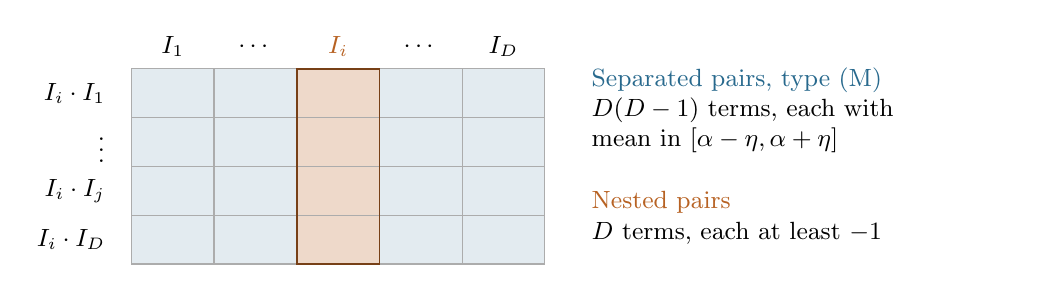
\begin{tikzpicture}[x=1.05cm,y=0.62cm,font=\small]
  \foreach \x in {0,1,2,3,4} {
    \foreach \y in {0,1,2,3} {
      \fill[parentblue!13] (\x,\y) rectangle +(1,1);
    }
  }
  \fill[childorange!24] (2,0) rectangle (3,4);
  \draw[gray!65,thin] (0,0) grid[xstep=1,ystep=1] (5,4);
  \draw[childorange!65!black,semithick] (2,0) rectangle (3,4);
  \node at (0.5,4.45) {$I_1$};
  \node at (1.5,4.45) {$\cdots$};
  \node[childorange] at (2.5,4.45) {$I_i$};
  \node at (3.5,4.45) {$\cdots$};
  \node at (4.5,4.45) {$I_D$};
  \node[anchor=east] at (-0.2,3.5) {$I_i\cdot I_1$};
  \node[anchor=east] at (-0.2,2.5) {$\vdots$};
  \node[anchor=east] at (-0.2,1.5) {$I_i\cdot I_j$};
  \node[anchor=east] at (-0.2,0.5) {$I_i\cdot I_D$};
  \node[anchor=west,align=left,text width=5.2cm] at (5.45,3.15)
    {\textcolor{parentblue}{Separated pairs, type (M)}\\
     \(D(D-1)\) terms, each with\\
     mean in \([\alpha-\eta,\alpha+\eta]\)};
  \node[anchor=west,align=left,text width=5.2cm] at (5.45,0.95)
    {\textcolor{childorange}{Nested pairs}\\
     \(D\) terms, each at least \(-1\)};
\end{tikzpicture}
\caption{The mixed term for fixed \(i\): the \((j,k)\) entry is
\(\ip{X_{I_i\cdot I_j}}{X_{I_k}}\). Rows index the children of \(I_i\),
columns index all parents; the grid is schematic. Only column \(i\) contains
nested pairs, a fraction \(1/D\) of the \(D^2\) terms.}
\label{fig:mixed-pairs}
\end{figure}

\paragraph{Step 6: the variance estimate.}
\emph{Claim:}
\begin{equation}\label{avg:variance}
  \mathbb E_A\norm{z_i-m}^2
    \leq\frac4D+4\left(1-\frac1D\right)\eta
    \qquad(1\leq i\leq D).
\end{equation}
Expand \(\norm{z_i-m}^2=\norm{z_i}^2-2\ip{z_i}{m}+\norm{m}^2\), average over
\(A\), and insert \eqref{avg:parent-bound}--\eqref{avg:mixed-bound}:
\[
 \mathbb E_A\norm{z_i-m}^2
 \le2\Bigl[\Bigl(1-\frac1D\Bigr)(\alpha+\eta)+\frac1D\Bigr]
   -2\Bigl[\Bigl(1-\frac1D\Bigr)(\alpha-\eta)-\frac1D\Bigr]
 =4\Bigl(1-\frac1D\Bigr)\eta+\frac4D .
\]
The terms in \(\alpha\) cancel exactly.

\paragraph{Step 7: conclusion.}
Average \eqref{avg:displacement} over \(g\in A\); the left side is the
constant \(\delta^2\). Then apply \eqref{avg:variance} to each of the \(D\)
summands:
\[
  \delta^2
  \leq\frac{L^2}{D}\sum_{i=1}^D \mathbb E_A\norm{z_i-m}^2
  \leq L^2\left(\frac4D+4\left(1-\frac1D\right)\eta\right).
\]
Since \(D\ge2\), \(1-1/D>0\), and solving for \(\eta\) gives
\(\eta\ge(\delta^2/L^2-4/D)/(4(1-1/D))=c_0\). The numerator is positive
exactly because \(D>4L^2/\delta^2\), which is \eqref{color:parameters}. The
constant \(c_0\) does not involve \(A\) or \(n\).
\end{proof}

\begin{proof}[Proof of \cref{thm:main}]
Suppose \(F\) were amenable. Apply the F\o lner criterion
\eqref{eq:folner} to the finite set \(S\) of \cref{sec:boundary} and
\(\varepsilon=c_0>0\) from \eqref{avg:boundary-bound}. It yields a nonempty
finite \(A\subset F\) with \(|hA\mathbin{\triangle}A|/|A|<c_0\) for all
\(h\in S\), contradicting \cref{avg:boundary}. Hence \(F\) is not amenable.
\end{proof}

\begin{remark}[Where each hypothesis enters; not part of the proof]
\label{rem:hypotheses}
(a) The group \(F\) enters only through \cref{dyad:eventual} and
\cref{dyad:transport}. The decisive property is that \emph{one} element moves
\emph{two} separated intervals of unrelated sizes and positions affinely onto
\(I_1\) and \(I_2\) at once. This is what makes the cross-correlations of
types (P), (S), (M) comparable in Step~2, and all three types are needed for
the cancellation of \(\alpha\) in Step~6. For comparison, in a group of
homeomorphisms of \(\R\) all of whose elements are affine, such as the
solvable and hence amenable group of maps \(x\mapsto2^kx+b\) with \(b\)
dyadic, an element is determined by its restriction to one interval. The
analogue of \cref{dyad:transport} fails there, Step~2 is unavailable, and
the argument gives nothing.

(b) Infinite dimension enters only through \cref{lem:displacement}. If
\(\dim H<\infty\), Brouwer's theorem forces \(\delta=0\) and
\eqref{avg:boundary-bound} is void.

(c) The Lipschitz property of \(f\) is used only in the last line of
\eqref{avg:displacement}. The inner product is used to form the scalar
functions \(\varphi_{I,J}\), to which the scalar inequality
\eqref{eq:finite-translation} applies.
\end{remark}

\section{Consequences}\label{sec:consequences}

This section is not used in the proof of \cref{thm:main}. Both corollaries
are obtained by inserting \cref{thm:main} into theorems of two companion
manuscripts. Those theorems are cited but not stated in the source, so the
deductions cannot be checked from the present text.

\subsection{Uniformly bounded representations}

\begin{corollary}\label{cor:nonunitarizable}
For every \(\varepsilon>0\), there are a separable complex Hilbert space
\(\mathcal H\) and a representation \(\pi:F\to\mathrm{GL}(\mathcal H)\) such
that \(\sup_{g\in F}\norm{\pi(g)}\le1+\varepsilon\), but no bounded invertible
operator \(V\) on \(\mathcal H\) makes every \(V\pi(g)V^{-1}\) unitary.
\end{corollary}

\begin{proof}[Proof, as given in the source]
The group \(F\) is countable: an element is determined by a finite list of
dyadic breakpoints and integer slope exponents. It is nonamenable by
\cref{thm:main}. The conclusion is then quoted from the companion
unitarizability theorem \cite[Theorem~1.1]{OpenAIUnitarizability2026}.
\unverified{The source does not reproduce the statement of
\cite[Theorem~1.1]{OpenAIUnitarizability2026}, and I could not consult it.
The deduction is valid only if that theorem gives exactly the displayed
conclusion, including the bound \(1+\varepsilon\), for every countable
nonamenable group. To my knowledge that general statement is the Dixmier
unitarizability problem, which was open in the literature I know, so this
corollary is conditional on the companion paper.}
\end{proof}

\subsection{Percolation on Cayley graphs}

Notation for this subsection only. Let
\(\Sigma\subset F\setminus\{\id\}\) be a finite symmetric generating set and
\(\mathrm{Cay}(F,\Sigma)\) the simple undirected Cayley graph with vertex set
\(F\) and edges \(\{g,g\sigma\}\), \(\sigma\in\Sigma\). In Bernoulli bond
percolation each edge is independently open with probability \(p\), under the
law \(\mathbb P_p\). Write \(p_c\) for the threshold for existence of an
infinite open cluster and \(p_u\) for the threshold for almost-sure uniqueness
of the infinite open cluster. The connection kernel
\(\mathcal C_p(g,g')=\mathbb P_p(g\leftrightarrow g')\) acts on
counting-measure \(\ell^2(F)\), initially on finitely supported functions by
summation over \(g'\). Put
\(p_{2\to2}=\sup\{p\in[0,1]:\mathcal C_p\text{ is bounded on }\ell^2(F)\}\).

\begin{corollary}\label{cor:percolation}
For every such generating set \(\Sigma\),
\[
  \norm{\mathcal C_{p_c}}_{2\to2}<\infty,\qquad p_c<p_{2\to2}\le p_u.
\]
For each fixed \(p\in(p_c,p_u)\), there are almost surely infinitely many
infinite open clusters. Moreover, there are deterministic numbers
\(p_c<p_1<p_2<1\), depending on \(\Sigma\), with the following property.
Couple all values of \(p\) by giving the edges independent uniform \([0,1]\)
labels and declaring an edge open at level \(p\) when its label is at most
\(p\). Then, with probability one, the level-\(p\) configuration has
infinitely many infinite open clusters simultaneously for every
\(p\in[p_1,p_2]\); that is, a single almost-sure event works for all these
\(p\).
\end{corollary}

\begin{proof}[Proof, as given in the source]
Apply the companion percolation result
\cite[Corollary~1.2]{OpenAIPercolation2026} to \(F\), which is nonamenable by
\cref{thm:main}.
\unverified{The source does not reproduce the statement of
\cite[Corollary~1.2]{OpenAIPercolation2026}, and I could not consult it. All
the conclusions (\(\norm{\mathcal C_{p_c}}_{2\to2}<\infty\), the strict
inequality \(p_c<p_{2\to2}\), the interval \([p_1,p_2]\)) come from that
result. To my knowledge \(p_c<p_u\) for Cayley graphs of arbitrary nonamenable
groups was an open conjecture in the literature I know, so this corollary is
conditional on the companion paper.}
\end{proof}

\appendix
\section{An explicit map with positive displacement}\label{app:auxiliary}

This appendix proves the Hilbert-space instance of
\cref{lem:displacement} \cite{BenyaminiSternfeld1983} directly. It is
independent of \cref{sec:proof} and its notation is used only here.

\begin{proposition}\label{aux:map}
Let \(H=L^2([0,1];\R^2)\), a real Hilbert space, and
\(B=\{x\in H:\norm{x}\le1\}\). There is a globally Lipschitz map
\(f:B\to B\) such that
\[
  \norm{f(x)}=1,
  \qquad \norm{f(x)-x}\ge\frac12
  \quad(x\in B).
\]
\end{proposition}

\paragraph{Plan.}
We construct a Lipschitz map \(\Phi:B\to H\) with
\(\inf_B\norm{\Phi}>0\) and \(\Phi(x)=x\) whenever \(\norm{x}\ge1/2\); then
\(f=-\Phi/\norm{\Phi}\) works. The identity map fails only because it vanishes
at \(0\). We modify it inside a thin tube around a curve \(\gamma\) through
\(0\): along the core of the tube the coefficient of \(\gamma\) is pushed down
to at most \(-1/8\), for all parameters \(t\ge-1\). This requires a curve that
stays in the ball of radius \(5/16\) for all \(t\ge1\) yet never comes close
to itself. Such a curve exists in infinite dimensions (\cref{aux:sep}). The
steps are: calculus of \(\gamma\) (\cref{aux:calc}); separation
(\cref{aux:sep}); nearest-point projection in a tube (\cref{aux:tube});
rotations aligning the tangent with the radial direction
(\cref{aux:rotation}); the map \(\Phi\).

\subsection{The curve}

For \(\xi=(\xi_1,\xi_2)\in\R^2\) put \(\xi^\perp=(-\xi_2,\xi_1)\), a linear
isometry with \(\xi^\perp\cdot\xi=0\). Put
\(\cvec(\vartheta)=(\cos\vartheta,\sin\vartheta)\), so that
\(\cvec'=\cvec^\perp\) and \(\cvec''=-\cvec\). Define functions on \(\R\) by
\[
 a(t)=
 \begin{cases}
 t/8,&t\le2,\\
 5/16-(3-t)^2/16,&2<t<3,\\
 5/16,&t\ge3,
 \end{cases}
 \qquad
 \theta(t)=
 \begin{cases}
 0,&t\le1,\\
 (t-1)^2/2,&1<t<2,\\
 t-3/2,&t\ge2,
 \end{cases}
\]
and, for \(w\in[0,1]\),
\[
 v(t)(w)=\cvec(\theta(t)w),\qquad
 \hat v(t)(w)=w\,\cvec(\theta(t)w)^\perp,
 \qquad \gamma(t)=a(t)v(t).
\]
Direct inspection gives the following facts.
\begin{enumerate}[label=(F\arabic*)]
\item\label{F1} \(a\) is continuous (\(a(2)=1/4\), \(a(3)=5/16\) from both
sides) and differentiable, with \(a'=1/8\) on \((-\infty,2]\),
\(a'(t)=(3-t)/8\) on \([2,3]\), and \(a'=0\) on \([3,\infty)\). Hence
\(0\le a'\le1/8\), \(a'\) is \(\tfrac18\)-Lipschitz, \(a\) is strictly
increasing on \((-\infty,3]\), \(a\le5/16\) everywhere, \(a(t)\ge1/8\) for
\(t\ge1\), \(a(t)\ge1/4\) for \(t\ge2\), and \(a(t)\le-1/8\iff t\le-1\).
\item\label{F2} \(\theta\) is continuous (\(\theta(2)=1/2\) from both sides)
and differentiable, with \(\theta'=0\) on \((-\infty,1]\),
\(\theta'(t)=t-1\) on \([1,2]\), and \(\theta'=1\) on \([2,\infty)\). Hence
\(0\le\theta'\le1\), \(\theta\) and \(\theta'\) are \(1\)-Lipschitz,
\(\theta=0\) on \((-\infty,1]\), \(\theta\) is strictly increasing on
\([1,\infty)\), and \(\theta(t)\to\infty\).
\item\label{F3} \(\norm{v(t)}=1\), \(\norm{\hat v(t)}^2=\int_0^1w^2\,dw=1/3\),
\(\ip{v(t)}{\hat v(t)}=0\), and \(\norm{\gamma(t)}=|a(t)|\). For \(t\le1\),
\(v(t)\) is the constant function \((1,0)\) and \(\gamma(t)=(t/8)v(t)\) is a
straight line through \(\gamma(0)=0\). For \(t\ge1\),
\(\norm{\gamma(t)}\le5/16\).
\end{enumerate}

\begin{lemma}[Calculus of the curve]\label{aux:calc}
\begin{enumerate}[label=(\roman*)]
\item \(v\) and \(\hat v\) are \(1\)-Lipschitz maps \(\R\to H\), and \(v\) is
differentiable in \(H\) with \(v'(t)=\theta'(t)\hat v(t)\).
\item \(\gamma\) is differentiable in \(H\), with
\[
 \gamma'(t)=a'(t)v(t)+a(t)\theta'(t)\hat v(t),
 \qquad
 \norm{\gamma'(t)}^2=a'(t)^2+\frac{a(t)^2\theta'(t)^2}{3}.
\]
\item \(c:=\inf_t\norm{\gamma'(t)}=\frac18\), and
\(M_\gamma:=\sup_t\norm{\gamma'(t)}\le\frac14\). Consequently \(\gamma\) is
\(M_\gamma\)-Lipschitz.
\item \(\gamma'\) is Lipschitz, with constant \(K_\gamma\le1\).
\item The unit tangent \(u(t)=\gamma'(t)/\norm{\gamma'(t)}\) is Lipschitz with
constant \(K_u\le16\); \(\ip{u(t)}{v(t)}=a'(t)/\norm{\gamma'(t)}\ge0\); and
\(u(t)=v(t)\) for \(t\le1\).
\item \(\ip{v(\tau)}{v(t)}=\sinc(\theta(t)-\theta(\tau))\), where
\(\sinc(\omega)=\sin(\omega)/\omega\) for \(\omega\ne0\) and \(\sinc(0)=1\).
\end{enumerate}
\end{lemma}

\begin{proof}
(i) Fix \(t,\tau\in\R\) and \(w\in[0,1]\), and put
\(\vartheta_0=\theta(t)w\), \(\vartheta_1=\theta(\tau)w\). By \ref{F2},
\(|\vartheta_1-\vartheta_0|\le|\tau-t|\). Since \(|\cvec'|=1\),
\(|\cvec(\vartheta_1)-\cvec(\vartheta_0)|\le|\tau-t|\); this bounds both
\(|v(\tau)(w)-v(t)(w)|\) and \(|\hat v(\tau)(w)-\hat v(t)(w)|\) (as
\(w\le1\)). Integrating the squares over \(w\) gives the two Lipschitz claims.
For the derivative, Taylor's formula with \(|\cvec''|=1\) gives
\(|\cvec(\vartheta_1)-\cvec(\vartheta_0)
-(\vartheta_1-\vartheta_0)\cvec(\vartheta_0)^\perp|
\le(\vartheta_1-\vartheta_0)^2/2\le(\tau-t)^2/2\). Since \(\theta'\) is
\(1\)-Lipschitz,
\(|(\vartheta_1-\vartheta_0)-(\tau-t)\theta'(t)w|
=w|\theta(\tau)-\theta(t)-(\tau-t)\theta'(t)|\le(\tau-t)^2/2\). Adding,
\[
 \bigl|v(\tau)(w)-v(t)(w)-(\tau-t)\theta'(t)\hat v(t)(w)\bigr|\le(\tau-t)^2
 \qquad\text{for every }w\in[0,1].
\]
The bound is uniform in \(w\), so
\(\norm{v(\tau)-v(t)-(\tau-t)\theta'(t)\hat v(t)}\le(\tau-t)^2\). This is
differentiability in \(H\).

(ii) The product rule for the \(C^1\) scalar \(a\) and the differentiable
\(H\)-valued \(v\) gives the formula for \(\gamma'\). The norm follows from
\ref{F3} (\(v\perp\hat v\), \(\norm{v}=1\), \(\norm{\hat v}^2=1/3\)).

(iii) \emph{Lower bound.} For \(t\le2\), \(a'(t)=1/8\), so
\(\norm{\gamma'(t)}^2\ge1/64\), with equality for \(t\le1\) where
\(\theta'=0\). For \(t\ge2\), \(a(t)\ge1/4\) and \(\theta'(t)=1\), so
\(\norm{\gamma'(t)}^2\ge a(t)^2/3\ge1/48>1/64\); this covers both \((2,3)\)
and \([3,\infty)\). \emph{Upper bound.} \(a'^2\le1/64\). The product
\(a\theta'\) vanishes for \(t\le1\), and for \(t\ge1\) satisfies
\(0\le a\theta'\le5/16\). So
\(\norm{\gamma'}^2\le1/64+25/768=37/768<1/16\). \emph{Lipschitz.} For a unit
vector \(\zeta\in H\), the scalar function \(t\mapsto\ip{\gamma(t)}{\zeta}\)
has derivative of absolute value at most \(M_\gamma\). By the mean value
theorem \(|\ip{\gamma(t)-\gamma(\tau)}{\zeta}|\le M_\gamma|t-\tau|\); take the
supremum over \(\zeta\).

(iv) For a bounded Lipschitz scalar \(\phi\) and a bounded Lipschitz
\(H\)-valued \(W\),
\(\Lip(\phi W)\le\Lip(\phi)\sup\norm W+\sup|\phi|\Lip(W)\). With
\(\phi=a'\), \(W=v\): \(\Lip(a'v)\le\frac18+\frac18\). The scalar
\(a\theta'\) is continuous, vanishes on \((-\infty,1]\), which is where \(a\)
is unbounded, and on each of \((1,2),(2,3),(3,\infty)\) has derivative
\(a'\theta'+a\theta''\) with \(|a'\theta'|\le1/8\) and \(|a\theta''|\le5/16\)
(as \(\theta''\in\{0,1\}\)). So \(\Lip(a\theta')\le7/16\) and
\(\sup|a\theta'|\le5/16\). With \(\phi=a\theta'\), \(W=\hat v\):
\(\Lip(a\theta'\hat v)\le\frac7{16}\cdot\frac1{\sqrt3}+\frac5{16}\). The
total is less than \(1\).

(v) For vectors with \(\norm x,\norm y\ge c\),
\[
 \Bigl\|\frac{x}{\norm x}-\frac{y}{\norm y}\Bigr\|
 \le\frac{\norm{x-y}}{\norm x}+\norm y\Bigl|\frac1{\norm x}-\frac1{\norm y}\Bigr|
 \le\frac{2\norm{x-y}}{c}.
\]
With \(c=1/8\) this gives \(K_u\le16K_\gamma\le16\). Next,
\(\ip{\gamma'}{v}=a'\norm v^2+a\theta'\ip{\hat v}{v}=a'\ge0\). For \(t\le1\),
\(\gamma'(t)=\frac18v(t)\), so \(u(t)=v(t)\).

(vi) Pointwise,
\(\cvec(\theta(\tau)w)\cdot\cvec(\theta(t)w)=\cos((\theta(t)-\theta(\tau))w)\),
and \(\int_0^1\cos(\omega w)\,dw=\sinc(\omega)\).
\end{proof}

\begin{lemma}[Injectivity and uniform separation]\label{aux:sep}
The curve \(\gamma\) is injective, and for every \(d>0\),
\begin{equation}\label{aux:separation}
 \sigma(d):=\inf_{|t-\tau|\ge d}\norm{\gamma(t)-\gamma(\tau)}>0 .
\end{equation}
\end{lemma}
This is what permits a tube of one fixed radius along the whole curve in
\cref{aux:tube}.

\begin{proof}
\emph{Injectivity.} Let \(\tau<t\) and suppose \(\gamma(\tau)=\gamma(t)\).
\begin{itemize}
\item If \(t\le1\): \(v(\tau)=v(t)\) is the same unit vector by \ref{F3}, so
\(a(\tau)=a(t)\), contradicting strict monotonicity of \(a\) on
\((-\infty,1]\).
\item If \(t>1\): by \ref{F2}, \(\theta(\tau)<\theta(t)\) (whether
\(\tau\le1\) or \(\tau>1\)). By \cref{aux:calc}(vi) and
\(|\sinc(\omega)|<1\) for \(\omega\ne0\),
\(|\ip{v(\tau)}{v(t)}|<1\), so the unit vectors \(v(\tau),v(t)\) are linearly
independent. Then \(a(\tau)v(\tau)=a(t)v(t)\) forces \(a(t)=0\),
contradicting \(a(t)\ge1/8\) for \(t\ge1\). This covers every sign of
\(a(\tau)\) and the range \(t,\tau\ge3\) where \(a\) is constant.
\end{itemize}

\emph{Separation.} Suppose \eqref{aux:separation} fails for some \(d\). Choose
\(\tau_n<t_n\) with \(t_n-\tau_n\ge d\) and
\(\norm{\gamma(t_n)-\gamma(\tau_n)}\to0\), and pass to a subsequence along
which \(\tau_n\to\tau_\infty\) and \(t_n\to t_\infty\) in \([-\infty,\infty]\).
Since \(\tau_n<t_n\), the possibilities are as follows.
\begin{itemize}
\item \emph{Both limits finite.} Then \(t_\infty-\tau_\infty\ge d\) and, by
continuity, \(\gamma(t_\infty)=\gamma(\tau_\infty)\), contradicting
injectivity.
\item \emph{Both \(-\infty\).} Eventually \(t_n,\tau_n\le1\), and then
\(\norm{\gamma(t_n)-\gamma(\tau_n)}=(t_n-\tau_n)/8\ge d/8\).
\item \emph{\(\tau_\infty=-\infty\), \(t_\infty>-\infty\).} Then
\(\norm{\gamma(\tau_n)}=|a(\tau_n)|\to\infty\) while
\(\norm{\gamma(t_n)}=|a(t_n)|\) stays bounded.
\item \emph{\(\tau_\infty\) finite, \(t_\infty=+\infty\).} Then
\(\theta(t_n)-\theta(\tau_n)\to\infty\), so
\(\ip{v(\tau_n)}{v(t_n)}\to0\) by \cref{aux:calc}(vi), and
\(\norm{\gamma(t_n)-\gamma(\tau_n)}^2
=a(t_n)^2+a(\tau_n)^2-2a(t_n)a(\tau_n)\ip{v(\tau_n)}{v(t_n)}
\to(5/16)^2+a(\tau_\infty)^2>0\).
\item \emph{Both \(+\infty\).} Eventually \(t_n,\tau_n\ge3\), so
\(a=5/16\) and \(\theta(t_n)-\theta(\tau_n)=t_n-\tau_n\ge d\), whence
\(\norm{\gamma(t_n)-\gamma(\tau_n)}^2
=2(5/16)^2\bigl(1-\sinc(t_n-\tau_n)\bigr)\). This is bounded away from \(0\)
because \(\sup_{\omega\ge d}\sinc(\omega)<1\): \(\sinc\) is continuous, less
than \(1\) on \((0,\infty)\), and tends to \(0\) at infinity.
\end{itemize}
Each case contradicts \(\norm{\gamma(t_n)-\gamma(\tau_n)}\to0\).
\end{proof}

\begin{lemma}[Tube and nearest-point projection]\label{aux:tube}
There is a radius \(0<\rho<1/32\) such that every point of
\[
 U=\{x\in H:\dist(x,\gamma(\R))<\rho\}
\]
has a unique nearest point \(\gamma(t(x))\) on the curve. Writing
\(e(x)=x-\gamma(t(x))\), we have \(\norm{e(x)}=\dist(x,\gamma(\R))<\rho\),
\(e(x)\perp u(t(x))\), and
\begin{equation}\label{aux:parameter}
 |t(x)-t(y)|\le16\norm{x-y}
 \quad\text{if }x,y\in U\text{ and }\norm{x-y}<\rho.
\end{equation}
\end{lemma}

\begin{proof}
\emph{Step 1 (tangent estimate).} Choose \(d>0\) with
\(K_\gamma d\le c/2=1/16\); \(d=1/16\) works by \cref{aux:calc}(iv).
\emph{Claim:}
\begin{equation}\label{aux:tangent}
 |\ip{\gamma(t)-\gamma(\tau)}{u(\tau)}|
 \ge\frac{3c}{4}|t-\tau|=\frac{3}{32}|t-\tau|
 \qquad(|t-\tau|\le d).
\end{equation}
Fix \(\tau\) and let \(\psi(t)=\ip{\gamma(t)}{u(\tau)}\). Then
\(\psi'(t)=\ip{\gamma'(t)}{u(\tau)}\) is \(K_\gamma\)-Lipschitz and
\(\psi'(\tau)=\norm{\gamma'(\tau)}\ge c\). Hence
\(|\psi(t)-\psi(\tau)-(t-\tau)\psi'(\tau)|
=|\int_\tau^t(\psi'(\varsigma)-\psi'(\tau))\,d\varsigma|
\le\frac{K_\gamma}2|t-\tau|^2\le\frac c4|t-\tau|\) when \(|t-\tau|\le d\), and
\eqref{aux:tangent} follows.

\emph{Step 2 (choice of \(\rho\)).} With \(\sigma(d)>0\) from \cref{aux:sep},
choose \(\rho>0\) such that
\begin{equation}\label{aux:radius}
 \rho<\frac1{32},\qquad 4\rho<\sigma(d),\qquad \rho K_u<\frac c4=\frac1{32}.
\end{equation}

\emph{Step 3 (a nearest point exists and \(e\perp u\)).} Let \(x\in U\) and
take \(t_n\) with \(\norm{x-\gamma(t_n)}\to\dist(x,\gamma(\R))<\rho\). For
large \(n\), \(\norm{x-\gamma(t_n)}<2\rho\), so any two late curve points are
less than \(4\rho<\sigma(d)\) apart. By the definition of \(\sigma(d)\) their
parameters differ by less than \(d\). So the late \(t_n\) lie in a compact
interval. A subsequence converges to some \(t_*\), and by continuity
\(\gamma(t_*)\) attains the distance. At any minimizing parameter \(t\), the
derivative of \(t\mapsto\norm{x-\gamma(t)}^2\), namely
\(-2\ip{x-\gamma(t)}{\gamma'(t)}\), vanishes; hence
\((x-\gamma(t))\perp u(t)\).

\emph{Step 4 (parameter estimate and uniqueness).} Let \(x,y\in U\) with
\(\norm{x-y}<\rho\). Let \(t\) be any minimizing parameter for \(x\), \(\tau\)
any for \(y\), and write \(x=\gamma(t)+e_t\), \(y=\gamma(\tau)+e_\tau\), with
\(\norm{e_t},\norm{e_\tau}<\rho\). Then
\(\norm{\gamma(t)-\gamma(\tau)}<3\rho<\sigma(d)\), so \(|t-\tau|<d\). Using
\(e_\tau\perp u(\tau)\) and \(e_t\perp u(t)\),
\[
 \ip{x-y}{u(\tau)}
 =\ip{\gamma(t)-\gamma(\tau)}{u(\tau)}+\ip{e_t}{u(\tau)-u(t)} .
\]
By \eqref{aux:tangent}, \(\norm{e_t}<\rho\), and \eqref{aux:radius},
\[
 \norm{x-y}\ge|\ip{x-y}{u(\tau)}|
 \ge\Bigl(\frac{3c}4-\rho K_u\Bigr)|t-\tau|\ge\frac c2|t-\tau|
 =\frac{|t-\tau|}{16}.
\]
Taking \(y=x\) shows that the minimizing parameter is unique. Then the same
inequality is \eqref{aux:parameter}.
\end{proof}

\begin{lemma}[Rotations]\label{aux:rotation}
There is a family of orthogonal operators \(R_t:H\to H\), \(t\in\R\),
Lipschitz in operator norm with some constant \(K_R\), such that
\(R_tu(t)=v(t)\) for all \(t\) and \(R_t=\mathrm{Id}\) for \(t\le1\).
\end{lemma}
It is used so that a residual \(e\perp u(t)\) is carried to a vector
perpendicular to \(v(t)\). Then changing the coefficient along \(v(t)\)
cannot be cancelled by the residual.

\begin{proof}
Fix \(t\), write \(u=u(t)\), \(v=v(t)\), and
\(\kappa=\ip uv\ge0\) (\cref{aux:calc}(v)). Define, for \(\zeta\in H\),
\[
 \Lambda\zeta=v\ip{u}{\zeta}-u\ip{v}{\zeta},
 \qquad R=\mathrm{Id}+\Lambda+\frac{\Lambda^2}{1+\kappa}.
\]
\emph{Case \(u,v\) linearly independent.} \(\Lambda\) is skew-adjoint,
vanishes on \(\{u,v\}^\perp\), and maps the plane \(\Pi=\mathrm{span}\{u,v\}\)
into itself, with \(\Lambda u=v-\kappa u\) and \(\Lambda v=\kappa v-u\). Hence
\(\Lambda^2u=\Lambda v-\kappa\Lambda u=-(1-\kappa^2)u\) and
\(\Lambda^2v=\kappa\Lambda v-\Lambda u=-(1-\kappa^2)v\), that is,
\(\Lambda^2=-(1-\kappa^2)\mathrm{Id}\) on \(\Pi\). So on \(\Pi\),
\(R=\bigl(1-\frac{1-\kappa^2}{1+\kappa}\bigr)\mathrm{Id}+\Lambda
=\kappa\,\mathrm{Id}+\Lambda\). This restriction satisfies
\((\kappa\mathrm{Id}+\Lambda)^*(\kappa\mathrm{Id}+\Lambda)
=\kappa^2\mathrm{Id}-\Lambda^2=\mathrm{Id}\) on \(\Pi\), so it is orthogonal
there, and \(Ru=\kappa u+v-\kappa u=v\). On \(\Pi^\perp\), \(R=\mathrm{Id}\).
Thus \(R\) is orthogonal on \(H\).

\emph{Case \(u,v\) linearly dependent.} Unit vectors with \(\ip uv\ge0\) that
are dependent are equal, so \(\Lambda=0\), \(R=\mathrm{Id}\), and \(Ru=v\). In
particular \(R_t=\mathrm{Id}\) for \(t\le1\).

\emph{Lipschitz dependence.} For parameters \(t,\tau\),
\(\norm{\Lambda_t-\Lambda_\tau}\le2(\norm{u(t)-u(\tau)}+\norm{v(t)-v(\tau)})
\le2(K_u+1)|t-\tau|\). Also \(\norm{\Lambda_t}\le2\), so
\(\norm{\Lambda_t^2-\Lambda_\tau^2}\le4\norm{\Lambda_t-\Lambda_\tau}\) and
\(\norm{\Lambda_t^2}\le4\). The scalar \(\kappa\) is \((K_u+1)\)-Lipschitz
and \(1+\kappa\ge1\), so \(1/(1+\kappa)\in(0,1]\) is
\((K_u+1)\)-Lipschitz. The product rule gives
\(K_R\le2(K_u+1)+8(K_u+1)+4(K_u+1)=14(K_u+1)\). The formula is the same in
both cases, so this holds also where \(u=v\).
\end{proof}

\subsection{Proof of Proposition~\ref{aux:map}}

Fix \(\rho\), \(U\), \(t(\cdot)\), \(e(\cdot)\) from \cref{aux:tube} and
\(R_t\) from \cref{aux:rotation}.

\paragraph{Step 0: definition of \(\Phi\).}
Set
\[
 b(t)=\min\{a(t),-1/8\},\qquad
 q(t)=b(t)-a(t)=-\max\{a(t)+1/8,0\}.
\]
By \ref{F1}: \(|q|\le5/16+1/8=7/16\), \(\Lip(q)\le\Lip(a)=1/8\), and
\(q(t)=0\) for \(t\le-1\). Let \(\beta,\chi:[0,\infty)\to[0,1]\) be
\[
 \beta(s)=
 \begin{cases}
 1,&s\le\rho/4,\\
 2-4s/\rho,&\rho/4<s<\rho/2,\\
 0,&s\ge\rho/2,
 \end{cases}
 \qquad
 \chi(s)=
 \begin{cases}
 1,&s\le\rho/2,\\
 2-2s/\rho,&\rho/2<s<\rho,\\
 0,&s\ge\rho,
 \end{cases}
\]
with \(\Lip(\beta)=4/\rho\), \(\Lip(\chi)=2/\rho\), and \(\beta\le\chi\).
Define \(\Phi:B\to H\) by \(\Phi(x)=x\) for \(x\in B\setminus U\), and, for
\(x\in B\cap U\) with \(t=t(x)\), \(e=e(x)\),
\begin{equation}\label{aux:G}
 \begin{split}
 \Phi(x)&=\bigl(a(t)+\beta(\norm e)q(t)\bigr)v(t)
       +\bigl((1-\chi(\norm e))\mathrm{Id}+\chi(\norm e)R_t\bigr)e\\
 &=x+\beta(\norm e)q(t)v(t)+\chi(\norm e)(R_t-\mathrm{Id})e ,
 \end{split}
\end{equation}
the two lines being equal because \(x=a(t)v(t)+e\).

\paragraph{Step 1: \(\Phi\) is Lipschitz on \(B\).}
We treat four kinds of pairs \(x,y\in B\).

\emph{(1a) \(x,y\in U\), \(\norm{x-y}<\rho\).} Write \(t,e\) for \(x\) and
\(\tau,e'\) for \(y\), and \(\Delta=\norm{x-y}\). From \cref{aux:tube} and
\cref{aux:calc}(iii):
\[
 |t-\tau|\le16\Delta,\qquad
 \norm{e-e'}\le\Delta+\norm{\gamma(t)-\gamma(\tau)}\le(1+16M_\gamma)\Delta,
 \qquad\bigl|\norm e-\norm{e'}\bigr|\le\Delta,
\]
the last because \(\norm{e(\cdot)}=\dist(\cdot,\gamma(\R))\) is
\(1\)-Lipschitz. For a product of three bounded Lipschitz factors, the
difference is at most the sum over factors of (variation of that factor)
\(\times\) (bounds of the other two). Apply this to the two correction terms
in the second line of \eqref{aux:G}.
\begin{itemize}
\item \(\beta(\norm e)\,q(t)\,v(t)\): bounds \(1\), \(7/16\), \(1\);
variations \(\frac4\rho\Delta\), \(\frac18\cdot16\Delta\), \(16\Delta\)
(\cref{aux:calc}(i)). Difference at most
\(\bigl(\frac{7}{4\rho}+2+7\bigr)\Delta\).
\item \(\chi(\norm e)\,(R_t-\mathrm{Id})\,e\): bounds \(1\), \(2\) (as
\(\norm{R_t}=1\)), \(\rho\); variations \(\frac2\rho\Delta\),
\(16K_R\Delta\), \((1+16M_\gamma)\Delta\). Difference at most
\(\bigl(4+16K_R\rho+2+32M_\gamma\bigr)\Delta\).
\end{itemize}
Hence \(\norm{\Phi(x)-\Phi(y)}\le C_1\norm{x-y}\) with
\(C_1=16+\frac7{4\rho}+16K_R\rho+32M_\gamma\).

\emph{(1b) \(\norm{x-y}\ge\rho\).} For \(x\in B\cap U\), \eqref{aux:G} gives
\(\norm{\Phi(x)}\le1+\frac7{16}+2\rho<\frac32\); outside \(U\),
\(\norm{\Phi(x)}\le1\). So
\(\norm{\Phi(x)-\Phi(y)}\le3\le\frac3\rho\norm{x-y}\).

\emph{(1c) \(x\in U\), \(y\notin U\), \(\norm{x-y}<\rho\).} For
\(0\le s<\rho\) we have \(\beta(s)\le\chi(s)\le2(\rho-s)/\rho\): with equality
on \([\rho/2,\rho)\), and because \(\rho-s\ge\rho/2\) on \([0,\rho/2]\). By
the second line of \eqref{aux:G},
\[
 \norm{\Phi(x)-x}\le\frac{2(\rho-\norm e)}{\rho}\Bigl(\frac7{16}+2\rho\Bigr)
 =\Bigl(\frac{7}{8\rho}+4\Bigr)(\rho-\norm e).
\]
Since \(\dist(y,\gamma(\R))\ge\rho\) and the distance function is
\(1\)-Lipschitz, \(\rho-\norm e\le\norm{x-y}\). With \(\Phi(y)=y\),
\(\norm{\Phi(x)-\Phi(y)}\le\bigl(\frac7{8\rho}+5\bigr)\norm{x-y}\).

\emph{(1d) \(x,y\notin U\).} \(\Phi\) is the identity.

These cases are exhaustive, so \(\Phi\) is Lipschitz with constant
\(C_\Phi=\max\{C_1,\frac3\rho,\frac7{8\rho}+5,1\}\).

\paragraph{Step 2: \(\norm{\Phi(x)}\ge\rho/4\) for all \(x\in B\).}
\emph{Outside \(U\):} since \(\gamma(0)=0\),
\(\norm x\ge\dist(x,\gamma(\R))\ge\rho\). \emph{Inside \(U\)}, use the first
line of \eqref{aux:G} and note that \(e\perp u(t)\) implies
\(R_te\perp R_tu(t)=v(t)\) and \(\norm{R_te}=\norm e\).
\begin{itemize}
\item \(\norm e\le\rho/4\): \(\beta=\chi=1\), so
\(\Phi(x)=b(t)v(t)+R_te\) with orthogonal summands, and
\(\norm{\Phi(x)}\ge|b(t)|\ge1/8>\rho/4\).
\item \(\rho/4<\norm e\le\rho/2\): \(\chi=1\), so \(\Phi(x)\) is a multiple
of \(v(t)\) plus \(R_te\perp v(t)\), and
\(\norm{\Phi(x)}\ge\norm e>\rho/4\).
\item \(\rho/2<\norm e<\rho\): \(\beta=0\), so
\(\Phi(x)=a(t)v(t)+e_*\) with
\(e_*=((1-\chi)\mathrm{Id}+\chi R_t)e\) and \(\norm{e_*}\le\norm e<\rho\). If
\(t>1\), then \(a(t)\ge1/8\) and
\(\norm{\Phi(x)}\ge1/8-\rho>3/32>\rho/4\). If \(t\le1\), then
\(R_t=\mathrm{Id}\), \(e_*=e\perp u(t)=v(t)\), and
\(\norm{\Phi(x)}\ge\norm e>\rho/2\).
\end{itemize}

\paragraph{Step 3: \(\Phi(x)=x\) whenever \(\norm x\ge1/2\).}
Outside \(U\) this is the definition. Inside \(U\),
\(|a(t)|=\norm{\gamma(t)}\ge\norm x-\norm e>\frac12-\rho>\frac{15}{32}
>\frac5{16}\). Since \(a\le5/16\) everywhere, \(a(t)<-5/16\). Hence
\(t\le-1\), so \(q(t)=0\) and \(R_t=\mathrm{Id}\), and the second line of
\eqref{aux:G} gives \(\Phi(x)=x\).

\paragraph{Step 4: the map \(f\).}
Define \(f(x)=-\Phi(x)/\norm{\Phi(x)}\) for \(x\in B\); this is legitimate by
Step~2, and \(\norm{f(x)}=1\). By the normalization inequality in the proof
of \cref{aux:calc}(v) with \(c=\rho/4\), \(y\mapsto y/\norm y\) is
\((8/\rho)\)-Lipschitz on \(\{\norm y\ge\rho/4\}\). With Step~1, \(f\) is
Lipschitz with constant \(8C_\Phi/\rho\). Displacement:
\begin{itemize}
\item if \(\norm x<1/2\), then
\(\norm{f(x)-x}\ge\norm{f(x)}-\norm x>1/2\);
\item if \(\norm x\ge1/2\), then \(\Phi(x)=x\) by Step~3, so
\(f(x)=-x/\norm x\) and
\(\norm{f(x)-x}=\norm x\,(1+1/\norm x)=1+\norm x\ge3/2\).
\end{itemize}
This proves \cref{aux:map}, and hence \cref{lem:displacement} with
\(\delta=1/2\). \qed

\section*{Verification checklist}

A sceptical reader should check these load-bearing points first.
\begin{enumerate}
\item \textbf{Exact covariance and its use} (\cref{dyad:covariancelemma};
Step~1 of \cref{avg:boundary}). Check that \(X_I(g)=X_{I_1}(h_{I,J}g)\) is an
exact equality of colors for every \(g\in A\). It needs \(hg=h\circ g\),
\(h\circ s_I=s_{I_1}\), and admissibility of both \(g\) and \(h_{I,J}g\) at
the \emph{same} level \(n\) (Step~0, via \cref{dyad:eventual}(b) applied to
\(A\cup SA\)).
\item \textbf{Pair transport} (\cref{dyad:transport}). Check that one element
of \(F\) moves both intervals affinely, and that all slopes are powers of
\(2\) after the bisections.
\item \textbf{Order of quantifiers} (\cref{sec:glance}, ``Order of choices'';
Step~0). \(S\) and \(c_0\) are fixed before \(A\); only \(n\) and \(\alpha\)
depend on \(A\); the final bound contains neither.
\item \textbf{The recursion identity \(X_{I_i}=f(z_i)\)} (Step~3). It rests
on \((T_{I_i})_{I_j}=T_{I_i\cdot I_j}\) (\cref{dyad:restrict}(c)) and on
well-foundedness of \eqref{color:recursion} (\cref{dyad:restrict}(b)).
\item \textbf{The variance computation} (Steps~5--6). Check which pairs are
separated (types (P), (S), (M) in \cref{sec:coloring}), that exactly \(D\) of
the \(D^2\) terms in each sum are not, and that \(\alpha\) cancels without
any sign assumption.
\item \textbf{The final inequality} (Steps~4 and~7). Line 2 of
\eqref{avg:displacement} uses \(m=\frac1D\sum_if(z_i)\); positivity of \(c_0\)
uses \(D>4L^2/\delta^2\).
\item \textbf{Existence of \(f\)} (\cref{app:auxiliary}). The delicate points
are the uniform separation \eqref{aux:separation} (\cref{aux:sep}, five limit
cases), the lower bound \(\norm{\Phi}\ge\rho/4\) (Step~2 of the proof of
\cref{aux:map}), and the Lipschitz estimate across the tube boundary (Step~1c
there). Alternatively, take \cref{lem:displacement} from
\cite{BenyaminiSternfeld1983}.
\item \textbf{The corollaries} (\cref{sec:consequences}) rest on companion
theorems not stated in the source; see the two boxed notes there.
\end{enumerate}

\bibliographystyle{plain}
\bibliography{sources}
\end{document}
